\section{对于源代码文件的说明}
本项目包含三个文件夹,分别是名为"lib"、"bin"和"src"的文件夹。

"lib"文件夹用于存放项目所需的第三方jar包,"bin"文件夹用于存放编译后的源代码字节码文件,"src"文件夹用于存放源代码。

在"src"文件夹中,分为客户端代码和服务端代码两个部分,即"Client"和"Server"文件夹。每个文件夹中包含四个Java文件,同时客户端和服务端各有一个主类用于运行,即"Main\_client"和"Main\_server"。

在"lib"文件夹中,包含两个客户端所依赖的第三方包,分别是"jxl-2.6.12.jar"和"itextpdf-5.5.8.jar"。
\newpage
\section{对于源代码中各个类的说明}
\subsection{Client文件夹中的类}
\subsubsection{Main\_client类}
这个类中使用了Java的图形用户界面(GUI)技术来创建一个客户端的主程序。具体来说,它使用了Java的AWT(Abstract Window Toolkit)和Swing库来实现用户界面的创建和显示。

代码中的Main\_client类的main方法是程序的入口点。在该方法中,通过创建一个UI对象,并传递参数"欢迎:"、300和200,来初始化一个用户界面。

UI类的构造函数接受标题、宽度和高度作为参数,并使用这些参数创建一个窗口。该窗口可能包含各种组件,如标签、按钮、文本框等,用于与用户进行交互和展示信息。

\subsubsection{Client类}
Client类只负责与服务端建立连接,之后将收到的数据发送到服务端。它向Worker类提供且只提供发送数据的功能。
这个类运用了Java中的网络编程技术,使用了Socket类和相关的输入输出流类来实现客户端与服务器之间的通信。

代码中的Client类具有一个构造函数,用于初始化客户端的名称和端口号。

Client类还定义了一个work方法,用于执行客户端的工作。该方法接收一个数据参数,将数据发送给服务器并接收服务器的响应。

在work方法中,通过创建一个Socket对象,使用指定的名称和端口号与服务器建立连接。然后通过获取套接字的输出流,使用DataOutputStream对其进行包装,以便将数据写入服务器。接着,通过获取套接字的输入流,使用DataInputStream对其进行包装,以便从服务器读取响应。最后,关闭与服务器的套接字连接,并返回从服务器接收到的响应。

\subsubsection{UI类}
UI类用来绘制图形操作界面,是客户端的主要部分,通过使用Worker类所提供的功能与用户交互。它包含了以下技术:

AWT (Abstract Window Toolkit): AWT是Java的原始窗口工具包,提供了创建图形用户界面(GUI)的基本组件和功能。代码中使用了java.awt包下的类,如java.awt.Frame和java.awt.event.ActionEvent。

Swing: Swing是Java的GUI工具包,提供了更多的GUI组件和更丰富的功能,用于创建富客户端应用程序。代码中使用了javax.swing包下的类,如javax.swing.JFrame、javax.swing.JButton和javax.swing.JPanel。

Event handling: 代码中实现了ActionListener接口,并重写了actionPerformed方法,用于处理按钮点击事件。

Layout management: 代码中使用了不同的布局管理器来布局界面,如null布局、GridLayout和CardLayout。

文本框和密码框:代码中使用了JTextArea来显示多行文本,JPasswordField来显示密码输入框。

通过上述技术,代码实现了一个基于Java的简单银行客户端界面。界面中包含了不同的窗口和按钮,实现了登录、注册、查询余额、取款、存款、转账、修改信息等功能。具体的界面和功能描述如下:

Frame1:初始界面,包含"登录"和"注册"按钮。

Frame2:登录界面,包含输入用户名和密码的文本框和登录按钮。

Frame3:用户界面,登录成功后显示,包含查询余额、取款、存款、转账、修改信息和销户等按钮。

Frame4:查询余额界面,显示当前用户余额和刷新按钮。

Frame5:取款界面,包含输入取款数目的文本框和取款按钮。

Frame6:存款界面,包含输入存款数目的文本框和存款按钮。

Frame7:转账界面,包含输入转入用户名和金额的文本框和转账按钮。

Frame8:修改信息界面,包含输入新密码、修改生日和手机号的文本框和修改按钮。

Frame9:注册界面,包含输入用户名、生日、手机号和密码的文本框和注册按钮。

Frame10:管理员界面,显示管理员操作界面,包含批量开户和年终报告按钮。

除了上述界面,代码中还包含了相关的按钮事件处理和布局管理的逻辑。

\subsubsection{Worker类}
这个类用于向UI类提供一些函数接口,这些函数实现了所要求的一些功能,并且通过发送一定格式的字符串来访问服务端数据库,Worker类与服务端的Operator类相对应。其中Worker类用来形成命令字符串,Operator类用来解析命令字符串。该类的编写过程主要运用了以下的Java编程技术:

文件操作技术:使用java.io.File类和java.io.FileOutputStream类来进行文件读写操作。

Excel文件读取技术:使用jxl.Workbook类和jxl.Sheet类来读取Excel文件中的数据。

异常处理技术:通过try-catch语句块处理可能发生的异常情况。

PDF文档操作技术:使用com.itextpdf.text.Document类和com.itextpdf.text.Paragraph类来创建和编辑PDF文档,以及使用com.itextpdf.text.pdf.PdfWriter类将文档写入文件。

这段代码的主要目标是实现一个银行系统的客户端功能。下面是该代码实现的功能:

Worker类的构造函数初始化了一个Client对象,用于与服务器建立连接。

check\_usr方法用于检查指定用户名是否存在于银行系统的数据库中。

check\_login方法用于判断指定用户名和密码是否匹配,即用于用户登录认证。

check\_money方法用于查询指定用户的账户余额。

withdraw\_money方法用于从指定用户的账户中取款,并返回操作是否成功。

store\_money方法用于向指定用户的账户中存款,并返回操作是否成功。

transfer方法用于将一位用户的资金转账给另一位用户,并返回操作是否成功。

signin方法用于注册一个新用户,并返回注册是否成功。

bulk\_signin方法用于批量注册多个新用户,从指定的Excel文件中读取用户信息,并返回成功注册的用户数量。

logout方法用于注销指定用户的账户,并返回操作是否成功。

update\_info方法用于修改指定用户的个人信息,如密码、生日和电话号码,并返回操作是否成功。

createpdf方法用于生成银行年度报告的PDF文件,包括总账户数、新增账户数和银行总资金,并返回操作是否成功。

但是其实代码中还存在一些潜在的缺陷。例如,异常处理部分仅仅是空的占位符,并没有实际处理可能发生的异常情况。此外,代码中的数据库操作涉及直接拼接SQL语句,存在安全风险和易受SQL注入攻击的问题。为了提高代码的健壮性和安全性,应该完善异常处理,并使用参数化查询或ORM框架来执行数据库操作。

\subsection{Server文件夹中的类}
\subsubsection{Main\_server类}
该类的目标是创建一个简单的服务器,通过监听指定的端口,接受客户端的连接请求,并为每个客户端连接创建一个新的线程来处理与客户端的通信。这种架构允许服务器同时处理多个客户端请求,提高了服务器的并发性能和响应能力。通过多线程的方式,服务器能够同时处理多个客户端的请求,而不会阻塞其他客户端的连接。

该类中的代码使用了Socket编程技术和多线程技术。

Socket编程技术:该代码创建了一个服务器端的Socket对象,并使用ServerSocket类在指定端口(6606)上监听客户端的连接请求。一旦有客户端连接成功,服务器将创建一个新的Socket对象来处理与该客户端的通信。

多线程技术:代码中的while循环用于不断接受客户端的连接请求。当有客户端连接成功后,代码通过创建新的线程来处理与该客户端的通信,从而实现了多个客户端之间的并发处理。每个客户端连接都在一个独立的线程中进行处理,以避免阻塞其他客户端的连接。

\subsubsection{Server类}
该类的目标是创建一个服务器,用于处理客户端发送的命令并提供相应的响应。服务器通过Socket编程实现与客户端的通信,接收客户端的连接请求,并根据客户端发送的命令执行相应的操作。根据命令的类型,服务器通过操作数据库(DB对象)执行数据库查询或更新操作,并将结果发送回客户端。多线程技术使服务器能够同时处理多个客户端连接,提高了服务器的并发性能和响应能力。

本类中也使用了Socket编程技术和多线程编程技术,除此之外还有:

输入输出流操作:代码使用DataInputStream和DataOutputStream来读取和写入数据。通过DataInputStream对象的readUTF()方法读取客户端发送的命令,并使用DataOutputStream对象的writeUTF()方法向客户端发送响应结果。

\subsubsection{DB类}
该类的目标是实现与MySQL数据库的连接和交互。它提供了数据库查询和更新的方法,通过执行传入的SQL语句,从数据库中获取查询结果或执行更新操作。使用JDBC技术,它允许Java应用程序与数据库进行通信和数据交换,实现了与数据库的交互功能。使用同步方法(synchronized)确保多线程环境下的线程安全性。

本类运用了以下技术:

JDBC(Java Database Connectivity):该类使用了JDBC技术来连接和操作数据库。它使用JDBC驱动程序(com.mysql.cj.jdbc.Driver)来连接MySQL数据库,并使用JDBC的API来执行SQL查询和更新操作。

数据库连接和操作:在DB类的构造函数中,它使用DriverManager类和getConnection()方法建立与MySQL数据库的连接。然后,它使用Statement对象(通过conn.createStatement()方法获得)执行SQL语句。通过调用executeQuery()方法执行查询操作,以获取结果集(ResultSet),并通过调用execute()方法执行更新操作。

异常处理:代码使用了异常处理机制来处理可能出现的SQL异常和其他异常。通过捕获和处理SQLException和Exception异常,它在发生错误时打印异常堆栈跟踪,提供了一定的错误处理和调试能力。

\subsubsection{Operator类}
该类的目标是解析命令字符串,从中提取出不同的部分,包括标志位(flag)、列名(column)和SQL语句。根据命令字符串的格式,它通过字符串处理和转换技术,将命令字符串拆分成相应的部分,以便后续使用。这些提取的部分可以用于执行数据库查询和更新操作,从而实现对数据库的操作。该类的方法提供了从命令字符串中获取不同部分的功能,以满足特定的操作需求。

本类运用了以下技术:

字符串处理:该类使用字符串处理技术来解析输入的命令字符串。它通过使用字符串的索引、子字符串和字符处理方法,提取出命令字符串中的各个部分。

字符串转换:代码使用了字符串转换技术来将字符转换为数字。通过调用parseInt()方法,它将字符型的数字转换为相应的整数值。
\newpage
\section{编译及运行}
\noindent1、准备工作
首先将服务端代码放入服务器(或虚拟机代替服务器),并在服务端创建相应的项目文件夹fmbank,在fmbank文件夹中创建存放字节码文件文件夹bin和源码文件夹src,将服务端代码Server文件夹放入src中。
\\\\
2、启动服务端程序
在服务端,首先进入项目文件fmbank,之后输入命令:
\\
\begin{adjustbox}{minipage=\linewidth, margin=0pt 0pt 2cm 0pt}
	\texttt{javac -encoding utf8 -d bin src/Server/*.java}
\end{adjustbox}
\\
编译java文件,并将class文件放入bin文件夹中。之后进入bin文件(相应命令:cd bin),输入:
\\
\begin{adjustbox}{minipage=\linewidth, margin=0pt 0pt 2cm 0pt}
	\texttt{java Server.Main\_server}
\end{adjustbox}
\\
启动程序,当屏幕输出如下提示表示程序运行成功。
\begin{figure}[htbp]
	\centering
	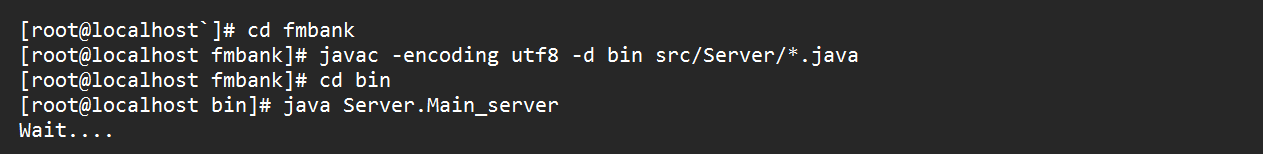
\includegraphics[width=0.8\textwidth]{figure/图1}
	\label{fig:example}
\end{figure}
3、启动客户端程序
首先进入项目文件fmbank,之后输入如下命令编译代码:
\\\\
\begin{adjustbox}{minipage=\linewidth, margin=0pt 0pt 2cm 0pt}
	\texttt{javac -encoding utf8 -d bin -cp .;lib\textbackslash jxl-2.6.12.jar;itextpdf-5.5.8.jar; src\textbackslash*Client\textbackslash*.java}
\end{adjustbox}
\\\\
其中-cp命令表示编译时引入第三方包。
之后进入bin文件,输入如下命令启动程序:
\\\\
\begin{adjustbox}{minipage=\linewidth, margin=0pt 0pt 2cm 0pt}
	\texttt{java -cp .;..\textbackslash lib\textbackslash jxl-2.6.12.jar;..\textbackslash lib\textbackslash itextpdf-5.5.8.jar; Client.Main\_client}
\end{adjustbox}
\\\\
出现如图界面表示启动成功:
\begin{figure}
	\centering
	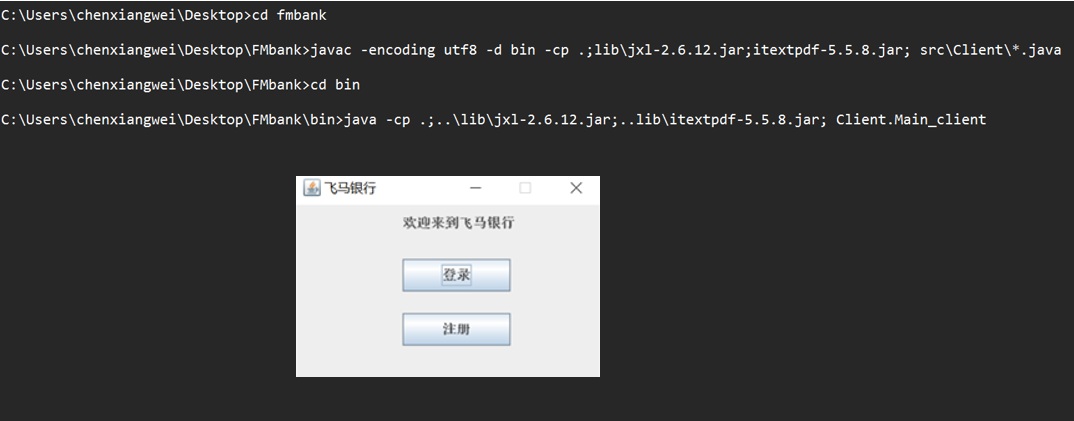
\includegraphics[width=0.8\textwidth]{figure/图2}
	\label{fig:example}
\end{figure}
\newpage
\section{结果展示}
1、注册功能\\
\begin{centering}
	\centering
	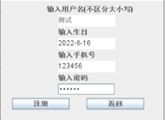
\includegraphics[width=0.8\textwidth]{figure/图3}
	\label{fig:example}
\end{centering}\\
\begin{centering}
	\centering
	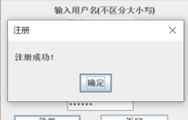
\includegraphics[width=0.8\textwidth]{figure/图4}
	\label{fig:example}
\end{centering}\\
2、登录功能\\
\begin{centering}
	\centering
	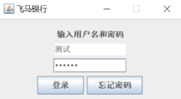
\includegraphics[width=0.8\textwidth]{figure/图5}
	\label{fig:example}
\end{centering}\\
\begin{centering}
	\centering
	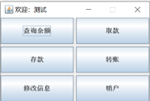
\includegraphics[width=0.8\textwidth]{figure/图6}
	\label{fig:example}
\end{centering}\\
3、查询功能\\
\begin{centering}
	\centering
	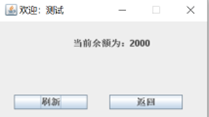
\includegraphics[width=0.8\textwidth]{figure/图7}
	\label{fig:example}
\end{centering}\\
4、存款功能\\
\begin{centering}
	\centering
	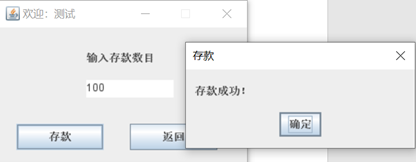
\includegraphics[width=0.8\textwidth]{figure/图8}
	\label{fig:example}
\end{centering}\\
\begin{centering}
	\centering
	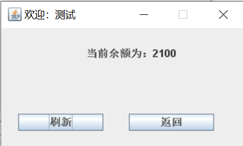
\includegraphics[width=0.8\textwidth]{figure/图9}
	\label{fig:example}
\end{centering}\\
5、取款功能\\
\begin{centering}
	\centering
	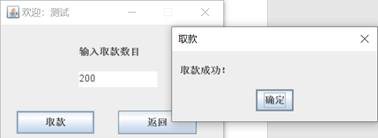
\includegraphics[width=0.8\textwidth]{figure/图10}
	\label{fig:example}
\end{centering}\\
\begin{centering}
	\centering
	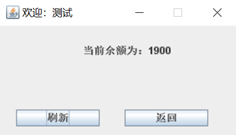
\includegraphics[width=0.8\textwidth]{figure/图11}
	\label{fig:example}
\end{centering}\\
6、转账功能\\
\begin{centering}
	\centering
	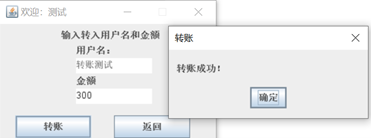
\includegraphics[width=0.8\textwidth]{figure/图12}
	\label{fig:example}
\end{centering}\\
\begin{centering}
	\centering
	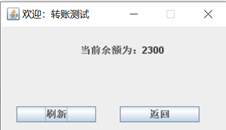
\includegraphics[width=0.8\textwidth]{figure/图13}
	\label{fig:example}
\end{centering}\\
7、销户功能\\
\begin{centering}
	\centering
	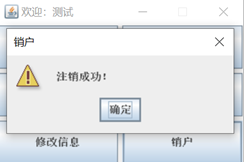
\includegraphics[width=0.8\textwidth]{figure/图14}
	\label{fig:example}
\end{centering}\\
8、报表功能\\
当用用户名root(管理员默认密码为八个八)登录时,会跳转到管理员界面,在管理员界面可以使用批量注册和生成报表功能。\\
\begin{centering}
	\centering
	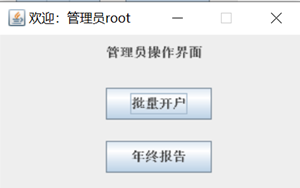
\includegraphics[width=0.8\textwidth]{figure/图15}
	\label{fig:example}
\end{centering}
